\part{Network protocols}
\chapter{TCP}

\textbf{TCP} is the most widely used Internet protocol.

Layer below: MAC layer ; layer above: APPlication layer

\section{Overview}

\begin{itemize}
  \item It is an end-to-end protocol (software only on the end hosts)
  \item It establishes a connection \dots
  \begin{itemize}
    \item reliable - with ACKnowledgements
    \item correct
    \item ordered - thanks to sequencing numbers
  \end{itemize}
  \item It is not so appropriate for current wireless scenarios (but there are
many variants of TCP)
  \item byte-stream oriented (app writes bytes - TCP sends segments - app
reads bytes)
\end{itemize}

\texttt{VEGAS}, \texttt{RENO}, \texttt{NEW RENO}, \texttt{SACK} are most
widely used TCP versions.

TCP does 2 types of control:

\begin{table}[h!]
  \begin{tabular}{c c}
  \hline
  \textbf{flow control} & avoid to overwhelm the receiver \\
  \hline
  \textbf{congestion control} & when there is a loss of packets, the flow
slows down \\
  \hline
  \end{tabular}
\end{table}

\section{Reliability in TCP}

Sequencing numbers are used to detect sequencing errors.

Timeouts are used to detect lost packets. \\

\textbf{Low RTO = Re-transmission TimeOut $\rightarrow$ Unneeded re-transmission}

\textbf{High RTO $\rightarrow$ Poor throughput} \\

Typically $RTO \simeq 4 RTT$; RTT = Round trip time. RTT determines the speed
of TCP connection.

\section{Fast Re-transmission}

\textbf{DUPlicate ACKs} are repeated ACKs for the same segment. Dup ACKs can
happen due to loss of packets, packets re-ordering, flow control window update.

Assuming that re-ordering is not so frequent, 3 or more Dup ACKs indicate a
loss and in this case there is no need to wait for a timeout to re-transmit
packet (this is the \textbf{fast re-transmission} and it is used to save time).

\section{Fast Recovery}

\textbf{Fast recovery} starts at SSTRESHold (\textbf{S}low \textbf{S}tart
\textbf{TRES}hold) and do additive increase after fast re-transmit.

Wireless problematics: the bandwidth is not fully used.

\section{Flow control}

\textbf{Palazzi Metaphor}: ``The bandwidth/capacity depends on the smallest
part of the pipe'' $pipeSize = Delay * Bandwidth$ \\

\textbf{Advertise window}: max number of bytes that the receiver can accepts \\

\textbf{Sending window}: actual bytes sent out = $min$(\textbf{congestion
window}, \textbf{advertise window})

\subsubsection{Additive Increase/Multiplicative Decrease}

\textbf{Purpose}: adjust to changes in the available capacity.

Congestion Window cwnd - handle flow of data in TCP connections (when
congestion goes down, increase cwnd, otherwise decrease it). \\

\texttt{MaxWin = min(CongestionWindow, AdvertisedWindow)}

\texttt{EffWin = MaxWin - (LastByteSent - LastByteAcked)} \\

How does the source determine if there is a congestion? It checks it with
timeouts and dupacks.

In general it is assumed that lost packet implies congestion but this is
not true in wireless environments!

In practice: increment a little for each ACK \dots

\begin{itemize}
  \item Increment = 1/cwnd
  \item cwnd += Increment
  \item cwnd = cwnd/2 if a timeout occurs
\end{itemize}

\begin{figure}[H]
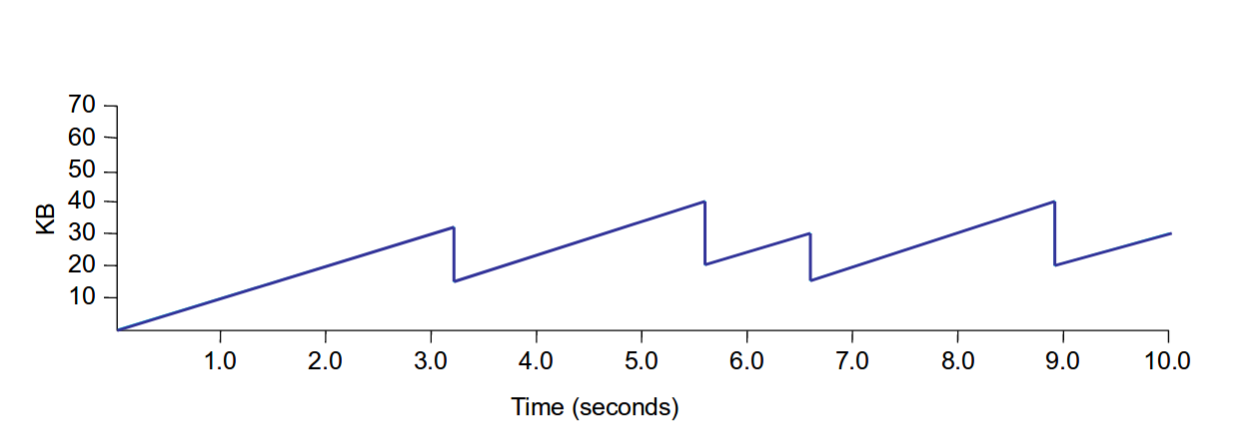
\includegraphics[scale=0.3]{sawtooth.png}
\caption{saw tooth shape behavior - timeouts cause \textbf{multiplicative
decrease (/2)}}
\end{figure}

\subsection{Slow Start Phase SS}

\textbf{Purpose}: quickly determine the available capacity.

This phase happens before addictive increase. It starts when first
starting connection or when connection goes dead waiting for timeout.

\begin{itemize}
  \item begin with cwnd = 1 packet
  \item \textbf{double (*2)} cwnd each RTT (increment by 1 packet for each ACK)
  \item This is exponential increase to check for available bandwidth
(up to half of cwnd may get lost)
\end{itemize}

This phase is not ``slow'', it is exponential!

\textbf{SSTHRESH} (slow start threshold) indicates when to begin additive
increase phase.

It is set to one half of cwnd on packet loss. So, SSTHRESH goes through
multiplicative decrease for each packet loss (because also the cwnd does so).
